

\id{ҒТАМР }\href{https://grnti.ru/?p1=06&p2=81&p3=65\#65}{06.81.65}
\begin{articleheader}

\sectionwithauthors{М.Д. Сайымова, Ғ.А. Мауина, А.С. Байдалинова, Г.М. Сағындықова}{ҚАЗАҚСТАН ЖАСТАРЫНЫҢ КӘСІПКЕРЛІК ОЙЛАУ ҚАБІЛЕТІН ДАМЫТУҒА ЫҚПАЛ ЕТЕТІН ЖӘНЕ КЕДЕРГІ КЕЛТІРЕТІН ФАКТОРЛАРДЫ ТАЛДАУ}

{\bfseries \textsuperscript{1}М.Д. Сайымова\textsuperscript{\envelope },
\textsuperscript{2}Ғ.А. Мауина, \textsuperscript{3}А.С. Байдалинова,
\textsuperscript{4}Г.М. Сағындықова}
\end{articleheader}
\begin{affiliation}
\textsuperscript{1}Ақтөбе өңірлік университеті. Қ. Жұбанова, Ақтөбе,
Қазақстан,

\textsuperscript{2}С. Сейфуллин атындағы Қазақ агротехникалық зерттеу
университеті, Астана, Қазақстан,

\textsuperscript{3}Esil University, Астана, Қазақстан,

\textsuperscript{4}Қ.Құлжанов атындағы Қазақ технология және бизнес
университеті», Астана қ, Қазақстан

\raggedright {\bfseries \textsuperscript{\envelope }}Корреспондент-автор: msaiymova@zhubanov.edu.kz
\end{affiliation}

Кәсіпкерлік кез келген елдің экономикалық дамуының маңызды аспектісі
болып табылады, әсіресе жұмыссыздық пен кедейлік сияқты күрделі
мәселелер әлі де сақталып отырған дамушы мемлекеттер үшін {[}1{]}.
Жоғары жұмыссыздық деңгейі, білім деңгейінің төмендігі және сыбайлас
жемқорлықтың кең таралуы жағдайында жастардың кәсіпкерлік ойлау
қабілетін қалыптастыру өте маңызды {[}1{]}. Оларға креативтілік,
тәуекелдерді басқару және проблемаларды шешу дағдылары сияқты негізгі
құзыреттерді бере отырып, кәсіпкерлік ойлау барлық мамандықтағы білім
алушылардың еңбек нарығындағы құндылығын айтарлықтай арттырады {[}2{]}.
{[}Кәсіпкерлік ойлауды дамыту бағдарламаларының танымалдығы артып келе
жатқанына қарамастан, олардың жастардың жұмыспен қамтылуы мен мансабына
ұзақ мерзімді әсерін зерттеу шектеулі болып қалуда {[}3{]}. Бұл мақала
осы олқылықтың орнын толтырып, Қазақстан Республикасындағы жастардың
кәсіпкерлік ойлау қабілетін қалыптастыруға әсер ететін факторлар мен
қазіргі жағдайды талдауды мақсат етеді.

Ғылыми мақалада кәсіпкерлік тұжырымдамасы бойынша қазіргі әдебиеттердің
жағдайы қорытындыланып, зерттеушілерге оның шығу тегі, тамыры мен
эволюциясын жақсы түсінуге мүмкіндік берді. Автор жастарды балалық
шақтан бастап кәсіпкер болуға шақырады. Өз күш-жігерінің нәтижесінде
олар кәсіпкерлік тәжірибені, дағдылар мен қабілеттерді, сондай-ақ
кәсіпкерлік қиындықтарды шешу қабілетін дамытады. Мақалада жастардың
кәсіпкерлік ойлау қабілетін дамыту алғышарттары талданады. Зерттеу
әдістері: Мақалада зерттеудің гипотезасы анықталғаннан бастап
қолданылған сауалнама және оған құрастырылған сұрақтар, оларды талдау
барысында статистикалық есетпеу тәсілдері авторлармен жүйелі қолданылды.

Кәсіпкерлік ойлаудың негізгі аспектілері бөлініп көрсетіледі.
Кәсіпкердің сыртқы және ішкі ортасының факторлары зерттеліп, олардың
ойлау тәсіліне және кәсіпкердің іс-әрекет ету тәсіліне әсері
негізделеді. Кәсіпкерлік ойлаудың дамуына қарай кәсіпкерліктің
эволюциясының негіздемелері мен бағыттары қалыптастырылады.

Кәсіпкерлікті жастар арасында насихаттаудағы осал тұстар анықталады.

{\bfseries Түйін сөздер:} кәсіпкерлік ойлау, жастар, кәсіпкерлік ойлаудың
эволюциясы, кәсіпкерлік, тұлғалық өсу, өзін-өзі жұмыспен қамту, шағын
және орта бизнес
\begin{articleheader}

{\bfseries АНАЛИЗ ФАКТОРОВ, СПОСОБСТВУЮЩИХ И ПРЕПЯТСТВУЮЩИХ РАЗВИТИЮ ПРЕДПРИНИМАТЕЛЬСКОГО МЫШЛЕНИЯ У МОЛОДЕЖИ КАЗАХСТАНА}

{\bfseries \textsuperscript{1}М.Д. Сайымова\textsuperscript{\envelope },
\textsuperscript{2}Г.А. Мауина, \textsuperscript{3}А.С. Байдалинова,
\textsuperscript{4}Г.М. Сагиндыкова}
\end{articleheader}
\begin{affiliation}

\textsuperscript{1}Актюбинский региональный университет имени
К.Жубанова, Актобе, Казахстан,

\textsuperscript{2}Казахский агротехнический исследовательский
университет им. С. Сейфуллина, Астана, Казахстан,

\textsuperscript{3}Esil University, Астана, Казахстан,

\textsuperscript{4}Казахский университет технологии и бизнеса им.
К.Кулажанова, Астана, Казахстан,

e-mail: msaiymova@zhubanov.edu.kz
\end{affiliation}

Предпринимательство является важным аспектом экономического развития
любой страны, особенно для развивающихся государств, где безработица и
бедность остаются серьезными проблемами {[}1{]}. В условиях высокого
уровня безработицы, низкого уровня образования и распространенной
коррупции крайне важно формирование предпринимательского мышления у
молодежи {[}1{]}. Предоставляя им ключевые компетенции, такие как
креативность, управление рисками и навыки решения проблем,
предпринимательское мышление значительно повышает ценность студентов
всех специальностей на рынке труда {[}2{]}. Несмотря на растущую
популярность программ по развитию предпринимательского мышления,
исследования их долгосрочного влияния на трудовую занятость и карьеру
молодежи остаются ограниченными {[}3{]}. Эта статья призвана восполнить
этот пробел, проанализировав текущее состояние и факторы, влияющие на
формирование предпринимательского мышления у молодежи в Республике
Казахстан.

В научной статье обобщено текущее состояние литературы по концепции
предпринимательства, что позволило исследователям лучше понять его
происхождение, корни и эволюцию. Автор призывает молодежь становиться
предпринимателями с детства. В результате своих усилий они развивают
предпринимательский опыт, навыки и способности, а также способность
решать предпринимательские трудности. В статье анализируются предпосылки
для развития предпринимательского мышления у молодежи.

В статье с момента формулировки гипотезы использовались анкетирование и
вопросы, разработанные для него, а также статистические методы анализа,
которые систематически применялись авторами.

Выделяются основные аспекты предпринимательского мышления. Исследуются
факторы внешней и внутренней среды предпринимателя, обосновывается их
влияние на образ мыслей и способ ведения деятельности предпринимателя.
По мере развития предпринимательского мышления формируются обоснования и
направления эволюции предпринимательства.

В заключении выявляются слабые стороны в пропаганде предпринимательства
среди молодежи.

{\bfseries Ключевые слова:} предпринимательское мышление, молодежь,
эволюция предпринимательского мышления, предпринимательство, личностный
рост, самозанятость, малый и средний бизнес.

\begin{articleheader}
{\bfseries ANALYSIS OF FACTORS FACILITATING AND HINDERING THE DEVELOPMENT OF ENTREPRENEURIAL THINKING AMONG THE YOUTH OF KAZAKHSTAN}

{\bfseries \textsuperscript{1}М.D. Saiymova, \textsuperscript{\envelope }
\textsuperscript{2}G.A. Mauina, \textsuperscript{3}A.S. Baidalinova,
\textsuperscript{4}G.M. Sagindykova}
\end{articleheader}
\begin{affiliation}

\textsuperscript{1}Aktobe Regional University named after K. Zhubanov
Акtobe, Kazakhstan,

\textsuperscript{2}S.Seifullin Kazakh Agro Technical Research
University, Astana, Kazakhstan,

\textsuperscript{3}Esil University, Astana, Kazakhstan,

\textsuperscript{4}K.Kulazhanov kazakh university of technology and
business, Astana, Kazakhstan,

e-mail: msaiymova@zhubanov.edu.kz
\end{affiliation}

Entrepreneurship is a vital aspect of the economic development of any
country, especially for developing nations where unemployment and
poverty remain serious issues {[}1{]}. In the context of high
unemployment rates, low education levels, and widespread corruption,
fostering entrepreneurial thinking among the youth is crucial {[}1{]}.
By providing key competencies such as creativity, risk management, and
problem-solving skills, entrepreneurial thinking significantly increases
the value of students from all disciplines in the labor market {[}2{]}.
Despite the growing popularity of programs aimed at developing
entrepreneurial thinking, studies on their long-term impact on youth
employment and career trajectories remain limited {[}3{]}. This article
seeks to fill this gap by analyzing the current state and factors
influencing the formation of entrepreneurial thinking among the youth in
the Republic of Kazakhstan.

The scientific article summarizes the current state of literature on the
concept of entrepreneurship, allowing researchers to better understand
its origins, roots, and evolution. The author encourages the youth to
become entrepreneurs from an early age. Through their efforts, they
develop entrepreneurial experience, skills, abilities, and the capacity
to address entrepreneurial challenges. The article analyzes the
prerequisites for developing entrepreneurial thinking among the youth.

From the formulation of the hypothesis, the article employed surveys and
questions developed for them, as well as statistical analysis methods
systematically applied by the authors.

The main aspects of entrepreneurial thinking are highlighted. The
factors of the external and internal environment of the entrepreneur are
studied, and their influence on the entrepreneur' s way
of thinking and approach to business activities is substantiated. As
entrepreneurial thinking evolves, justifications and directions for the
evolution of entrepreneurship are formulated.

In conclusion, the weak points in promoting entrepreneurship among the
youth are identified.

{\bfseries Keywords}: entrepreneurial thinking, youth, evolution of
entrepreneurial thinking, entrepreneurship, personal growth,
self-employment, small and medium-sized businesses.
\begin{multicols}{2}

{\bfseries Кіріспе.} Қазіргі таңда, инновациялар мен технологиялық
өзгерістермен толтырылған тез өзгеріп жатқан әлемде кәсіпкерлік
экономикалық және әлеуметтік прогрестің қозғаушы күші болып табылады.
Жастар арасында кәсіпкерлік ойлауды дамыту тек жеке өсу аспектісі ғана
емес, сонымен бірге қоғамның тұрақты дамуының негізгі элементі болып
табылады. Кәсіпкерлік кез келген елдің экономикалық дамуының маңызды
факторларының бірі болып табылады {[}1,4{]}. Ол тек жұмыс орындарын
құрып, халықтың табысын қамтамасыз етіп қана қоймай, сонымен қатар
инновацияларды ынталандырады, бұл өз кезегінде қоғамның әл-ауқатын
арттыруға ықпал етеді {[}1,4{]}.

Креативтілікпен, тәуекелге дайындықпен және инновацияларға
қабілеттілікпен сипатталатын кәсіпкерлік ойлау жас мамандардың еңбек
нарығындағы бәсекеге қабілеттілігін айтарлықтай арттыра алады, сондай-ақ
жаңа жұмыс орындарын құруға және елдің экономикалық негізін нығайтуға
ықпал етеді. Қазақстан Республикасында жастардың кәсіпкерлік әлеуетін
дамыту ерекше маңызға ие, өйткені мұнда жастар арасындағы жұмыссыздық
деңгейі дәстүрлі түрде жоғары, ал мамандық бойынша жұмысқа орналасу
мүмкіндіктері шектеулі {[}1,4{]}. Жастардың кәсіпкерлік ойлау қабілетін
қалыптастыру жұмыссыздық мәселелерін шешіп қана қоймай, өсіп келе жатқан
ұрпақтың шығармашылық және инновациялық әлеуетін жүзеге асыруға ықпал
етуі мүмкін.

Жоғары оқу орындарында кәсіпкерлікті оқыту осы процесте маңызды рөл
атқарады. Ол тек білім мен дағдыларды беріп қана қоймай, сонымен бірге
студенттердің сыни ойлау және өз бетінше шешім қабылдау қабілеттерін
қалыптастырады. Осы контексте әлемдегі университеттер кәсіпкерлік
құзыреттіліктерді дамытуға бағытталған түрлі бағдарламалар мен
курстарды, жеке модульдерден бастап толық бакалавриат және магистратура
бағдарламаларына дейін енгізуде.

Дүниежүзілік экономикалық форумның (WEF) 2008 жылы басталған жаһандық
білім беру бастамасы кәсіпкерлерді жаппай дайындаудың тұрақты әлеуметтік
даму мен экономикалық қалпына келтірудің негізгі элементі ретінде
маңыздылығын атап өтеді {[}WEF, 2009{]}. Қазақстанда бұл мәселе
экономика диверсификациясын және инновациялық қызметті ынталандыру
қажеттілігін ескере отырып, барған сайын өзекті бола түсуде.

Жас кәсіпкерлер құратын шағын және орта бизнес ел экономикасында маңызды
рөл атқарады, жұмыс орындарын құруға және жалпы әл-ауқатты арттыруға
ықпал етеді. Алайда, бұған қол жеткізу үшін жастар арасында кәсіпкерлік
ойлауды мақсатты түрде қалыптастыру қажет, бастапқы кезеңдерден бастап
және оқу процесі бойы жалғасады.

Бұл мақалада Қазақстан жастарының кәсіпкерлік ойлау қабілетін
қалыптастырудың алғышарттары мен шарттары талданады, кәсіпкерлік
қабілеттерді дамытуға әсер ететін ішкі және сыртқы факторлар зерттеледі
және кәсіпкерлік ойлаудың эволюциясының бағыттары негізделеді.
Зерттеудің мақсаты -- білім беру бағдарламаларына кәсіпкерлік пен
кәсіпкерлік ойлауды интеграциялаудың әдістемелік негіздерін құру, бұл
жаңа буын кәсіпкерлерін тәрбиелеуге мүмкіндік береді, олар заманауи
әлемнің сын-қатерлеріне тиімді бейімделе алады және шағын және орта
бизнестің, сондай-ақ жалпы ұлттық экономиканың дамуына елеулі үлес
қосады.

\begin{enumerate}
\def\labelenumi{\arabic{enumi}.}
\item
  {\bfseries Гипотеза 1:} Техникалық мамандық студенттері гуманитарлық
  мамандық студенттеріне қарағанда кәсіпкерлік қызметке жоғары дайындық
  көрсетеді.
\item
  {\bfseries Гипотеза 2:} Жыныс, жас және оқу ақысының төлем нысаны
  студенттердің тәуекелдерді қабылдауына және олардың кәсіпкерлік
  қызметке дайындығына айтарлықтай әсер етеді.
\item
  {\bfseries Гипотеза 3:} Білім беру бағдарламаларына жобалық қызмет пен
  практикалық бағытталған курстарды енгізу студенттердің кәсіпкерлік
  құзыреттерін белсенді дамытуға ықпал етеді. Студенттердің кәсіпкерлік
  жобаларын жүзеге асыру үшін инвесторларды іздеу процесін жандандыру
  қажет.
\end{enumerate}

Зерттеу нәтижелері студенттердің жасы, жынысы, оқу ақысының төлем нысаны
және мамандану бойынша деректердің талдауын қамтиды. Сауалнама
сұрақтарына жауаптардың семантикалық талдауы кәсіпкерлік ойлауға
байланысты жиі қолданылатын сөздер мен сөз тіркестерін анықтауға
мүмкіндік берді. Логистикалық регрессия көмегімен студенттердің
кәсіпкерлік ойлауына әсер ететін әртүрлі факторлардың маңыздылығы
бағаланды. Деректердің дәлдігін қамтамасыз ету үшін жоспарлар мен
тапсырмалардың уақтылы орындалуын бақылау қажет.

Маңызды регрессия коэффициенттерін интерпретациялау демографиялық
факторлардың және білім беру ортасының студенттердің кәсіпкерлік
ойлауына әсері туралы қорытынды жасауға мүмкіндік береді. Зерттеу
нәтижелерін гипотезалармен салыстыру бұл факторларды білім беру
бағдарламаларын әзірлеу кезінде ескерудің маңыздылығын растады.
Деректерді талдау мен интерпретациялау тәсілдерін неғұрлым дәл енгізу
механизмін күшейту қажет.

\emph{Әдебиетке шолу.} Көптеген зерттеулер жастар арасында кәсіпкерлік
ойлауды дамытудың жұмыссыздық мәселелерін шешу және инновациялық
белсенділікті ынталандыру жолы ретінде маңыздылығын көрсетеді.

Жас кәсіпкерлер жаңа технологияларды құруға және енгізуге, сондай-ақ
білім мен ғылымды дамытуға үлкен үлес қосады {[}5,6{]}. Алайда, бұл
тақырыптың маңыздылығы мойындалғанына қарамастан, Қазақстан
Республикасында жастардың кәсіпкерлік ойлау қабілетін қалыптастыру
ерекшеліктеріне арналған зерттеулер өте аз {[}6{]}.

Бұрын жүргізілген зерттеулер кәсіпкерлік ойлауды дамытатын бірнеше
факторларды анықтады. Мысалы, сапалы білімнің қолжетімділігі жастардың
кәсіби мобильділігінің және олардың табысты өзін-өзі жүзеге асыруының
маңызды элементі болып табылады {[}7{]}. Сондай-ақ қажетті
инфрақұрылымның, қаржылық ресурстардың және білікті кадрлардың
қолжетімділігі үлкен маңызға ие {[}6{]}. Сонымен қатар, кәсіпкерлік
ойлауды қалыптастыруға отбасылық мәртебе, ата-аналардың білім деңгейі,
кәсіпкерлік қызметке қатысу тәжірибесі сияқты факторлар әсер етуі мүмкін
{[}1{]}. Алайда, бұл факторлардың Қазақстан жастарының кәсіпкерлік ойлау
қабілетін дамытуға әсері жеткілікті түрде зерттелмеген.

Л. Босман және С. Фернхабер жеке құзыреттерді, ең алдымен кәсіпкерлік
ойлауды дамытудың ерекше маңыздылығын атап өтеді. Ойлау - бұл ақыл-ой
қондырғысы немесе бейімділік болғандықтан, кәсіпкерлік ойлау
"мүмкіндіктерді ашуға, бағалауға және пайдалануға бейімділік" ретінде
анықталады {[}8{]}.

Кәсіпкерлік ойлауды бизнесті бастау үшін ғана емес, оны ұйым ішіндегі
стратегиялық әрекеттер үшін де қолдануға болады. Үлкен немесе кіші
кәсіпорындар болсын, кәсіпкерлік ойлау барлық студенттерге,
мамандықтарына немесе қызметіне қарамастан, өзекті және қажетті болып
табылады. Жоғары білім беру саласындағы кәсіпкерлік барған сайын
кәсіпкерлік креативтілікті студенттердің инновациялық қабілеттерін
жақсартудың маңызды факторы ретінде бағалайды.

Шаньдун, Цзянсу және Чжэцзян провинцияларындағы кәсіпкерлік
университеттерді зерттеу барысында кәсіпкерлік білім беру мен
шығармашылықтың кәсіпкерлік ниеттерге оң және айтарлықтай әсер ететіні
анықталды. Сонымен қатар, нәтижелер кәсіпкерлік ойлау, шабыт және
өзін-өзі тиімділік арасындағы байланыс кәсіпкерлік білім беру мен
шығармашылықтың аралық байланысын көрсететінін көрсетті.

Кәсіпкерлік экономикалық өсуді ынталандыруда және экономикаға оң әсер
етуде маңызды рөл атқарады {[}9{]}. Кәсіпкерлер нарықтағы олқылықтарды
анықтап, пайдалануға қабілеттілігімен танымал {[}8{]}. Олар инновациялық
өнімдер, қызметтер мен процестерді әзірлейді, бұл технологиялық
прогреске әкеледі. Бұл өз кезегінде салалардағы өнімділікті, тиімділікті
және бәсекеге қабілеттілікті арттырып, экономикалық өсуді ынталандырады.

Бандура (1992) әзірлеген әлеуметтік когнитивтік теорияға сәйкес, адамның
өзін-өзі тиімділік деңгейі кәсіпкерлік білім алу арқылы артуы мүмкін.
Адамдарға кәсіпкерлік қызметке қатысу мүмкіндігі беріледі, мысалы,
мүмкіндіктерді іздеу, компанияның техникалық-экономикалық талдауын
жүргізу және нәтижесінде іс жүзінде қолданылатын бизнес-жоспарлар құру.
Бұрынғы зерттеулер кәсіпкерлікке оқыту, кәсіпкерлік ойлау және
креативтілік жас таланттарды дамытып, адамдарда кәсіпкерлік ниет
қалыптастыратынын көрсетті.

Жеке және қоғамдық деңгейде кәсіпкерлікпен байланысты артықшылықтар,
мысалы, өзін-өзі жұмыспен қамту мүмкіндіктерін құру, өмір сүру деңгейін
жақсарту және кедейлікті азайту, сондай-ақ басқа да әлеуметтік және
экономикалық өсудің түрлері бар екені айтылды.
\href{https://www.frontiersin.org/articles/10.3389/fpsyg.2023.1240910/full\#ref31}{Israr
and Saleem (2018)}, деректері бойынша, студенттер қазіргі уақытта
өзін-өзі жұмыспен қамтуды қалайды, бұл соңғы жылдары студенттер арасында
кәсіпкерліктің кәсібилік ретінде танымал болуының өсуіне ықпал етті.
Кәсіпкерлік ойлау әдетте табысты кәсіпкерлермен байланысты қатынастар,
мінез-құлық және ойлау тәсілдерінің жиынтығын білдіреді {[}8{]}.
Кәсіпкерлік ойлауды дамыту тек өз бизнесін бастайтындарға ғана
қолжетімді емес. Бұл сондай-ақ корпоративтік жағдайларда да пайдалы
болуы мүмкін, онда адамдар инновацияларды ынталандыру және мәселелерді
шешу үшін кәсіпкерлік ойлауды қолдана алады.
\href{https://www.frontiersin.org/articles/10.3389/fpsyg.2023.1240910/full\#ref51}{Rodrriguez
and Lieber (2020)} кәсіпкерлік ойлау кәсіпкерлік сектордағы
мүмкіндіктерді анықтау және пайдалану қабілетімен сипатталатынын айтады.

Кейбір теорияларға сәйкес, қоршаған орта адамдарға өз ойлауын оқыту
немесе тәжірибе арқылы дамытуға көмектесуі мүмкін, бұл кәсіпкерлік
білімнің маңыздылығын растайды.

Цифрландыру жағдайында цифрлық әлемде жұмыс істеу кезінде цифрлық
кәсіпкерлік ойлауды қабылдау қажеттілігі атап өтіледі.
Domino' s Tesco және Tate Art Galleries табыс тарихларын
талқылау деректерге, бұлттық технологияларға және платформаға
негізделген бизнес-әрекеттерді зерттеуге көмектеседі, цифрлық
кәсіпкерлік ойлауды дамыту цифрлық технологиялар дәуіріндегі табысқа
жету жолындағы алғашқы қадам болып табылады. Жалпы, жоғарыда аталған
жағдайлар цифрлық кәсіпкерлік ойлауға сүйенетін кәсіпорындар жақсы
қаржылық көрсеткіштерге қол жеткізетінін көрсетеді. Бұл компаниялардың
менеджерлері мен қызметкерлері цифрлық технологиялар арқылы ашылатын
мүмкіндіктерді анықтау, бағалау және пайдалану қабілетін көрсетті.

Кәсіпкерлік ойлау өмір бойы оқуға және тұрақты жеке және кәсіби өсуге
деген ұмтылысты арттырады. Кәсіпкерлік ойлауы бар адамдар кәсіпкерлікті
үздіксіз бейімделуді және оқытуды қажет ететін дамушы жол деп түсінеді.
Олар белсенді түрде жаңа білім іздейді, салалық үрдістерді қадағалайды
және жаңа идеялар мен перспективаларға ашық болады. Мұндай ойлау
кәсіпкерлік білім берудің тұрақты сипатына сәйкес келеді, адамдарды
формальды білім беру тәжірибесінен тыс оқуын жалғастыруға итермелейді.
Жалпы алғанда, кәсіпкерлік білім кәсіпкерлік ойлауды қалыптастыру мен
дамытуда маңызды рөл атқарады. Ол адамдарға табысты кәсіпкерлік үшін
қажетті білімді, дағдыларды, тәжірибені және қолдау жүйелерін ұсынады.
Ғылыми деректерге сәйкес, кәсіпкерлік ойлау адамның кәсіпкерлік қызметке
және нәтижелерге бағытталған мінез-құлық үлгілерін бағыттай отырып, оның
кәсіпкерлік мінез-құлқымен тығыз байланысты. Осылайша, білім беру
қатынасқа әсер етуі мүмкін, бұл өз кезегінде кәсіпкерлік ниеттерді
болжайды.

Практикалық түрде барлық зерттеушілер Й. Шумпетерге дейін кәсіпкердің
негізгі мотиві ретінде пайданы бөліп көрсетті. Австриялық және
америкалық экономист, әлеуметтанушы және экономикалық ой тарихшысы Йозеф
Шумпетер бірінші болып кәсіпкерлік белсенділіктің қозғаушы күші ретінде
пайданы алуды емес, инновациялық процесті ұсынды {[}10{]}

Сонымен бірге, кәсіпкердің жеке мотивация жүйесінде қызмет нәтижесінің
критерийлері (кіріс, қоғамдық мойындау, әлеуметтік мәртебе және т.б.)
емес, кәсіпкерлік қызмет процесінің факторлары (потенциалды ашу
мүмкіндіктері, жеке өсу, өзін-өзі табу, өмірдің мағынасын табу) шешуші
болып табылады

{\bfseries Материалдар мен әдістер.} Бұл зерттеу Қазақстан Республикасының
жастарының кәсіпкерлік ойлау қабілетін қалыптастыруға әсер ететін
негізгі факторларды анықтауға бағытталған. Осы мақсатқа жету үшін ғылыми
әдебиеттер, мемлекеттік статистика және сараптамалық бағалаулар
талданды. Бандураның (1992), әлеуметтік когнитивтік теориясына сәйкес,
адамның өзін-өзі тиімділік деңгейі, яғни оның өз қабілеттеріне деген
сенімі оның мінез-құлқы мен жетістіктеріне шешуші әсер етеді. Осылайша,
кәсіпкерлік ойлаудың маңызды компоненті - бұл өз күштері мен
қабілеттеріне деген сенімділік {[}5{]}.

Жеке сипаттамалардан басқа, кәсіпкерлік ойлауды қалыптастыруға
әлеуметтік-мәдени, институционалдық және экономикалық факторлар да әсер
етуі мүмкін. Осы факторлардың кешенді талдауы Қазақстан Республикасының
жастары арасындағы кәсіпкерлік ойлаудың қазіргі жағдайы мен даму
перспективалары туралы толығырақ түсінік алуға мүмкіндік береді. Алдыңғы
зерттеулер кәсіпкерлікті оқыту, кәсіпкерлік ойлау және креативтілік жас
таланттарды дамытып, адамдарда кәсіпкерлік ниетті қалыптастыратынын
көрсетті {[}2{]}. Осы мақсатта ресми статистикалық деректер, ғылыми
басылымдар және сараптамалық бағалаулар сияқты әртүрлі дереккөздерден
мәліметтер жиналды.

Мақала жазу үшін негізгі ақпарат көздері: теориялық деңгейде - зерттеу
мәселесіне арналған ғылыми мақалалар, монографиялар, мерзімді басылымдар
және басқа да жұмыстар; эмпирикалық деңгейде - ресми дереккөздердің
деректері, далалық зерттеулердің нәтижелері (ЖОО-ның барлық
курстарындағы студенттерді сауалнама).

Мақаланың мақсатына жету үшін жастар арасында кәсіпкерлік ойлауды дамыту
бойынша қайталама ақпараттарды жинау, ЖОО студенттерінің пікірлерін
анықтау, Қазақстан Республикасының жастарының кәсіпкерлік ойлауды
дамытуға арналған тиімді құралдарды анықтау сияқты сапалық және сандық
зерттеу әдістері қолданылды. Сапалық зерттеу әдістері ретінде кабинет
зерттеуі және сарапшылармен тереңдетілген сұхбаттар қолданылды.
Сарапшылар ретінде кәсіпкерлік курсының оқытушылары, бизнес-тренерлер,
аймақтағы белсенді кәсіпкерлер және аймақтық "Атамекен" Ұлттық
Кәсіпкерлер Палатасының өкілдері болды. Тереңдетілген сұхбаттар Ақтөбе
қаласында өткізілді.

Сонымен қатар, фокус-топ әдісі қолданылды. Зерттеу аясында әрқайсысында
8 адамнан тұратын 2 фокус-топ өткізілді. Фокус-топтың қатысушылары
кәсіпкерлікпен айналысатын студенттер, кәсіпкерлікпен айналысқысы
келетін студенттер, ЖОО түлектері - бизнес иелері болды. Әр топтың
ұзақтығы 1,5-2 сағатты құрады.

Студенттердің кәсіпкерлік ойлауды қалыптастыруы мен дамуын сандық
бағалау үшін бетпе-бет сауалнама жүргізілді. Респонденттерді таңдау ЖОО
факультеттері бойынша кездейсоқ іріктеу әдісімен жүргізілді.

Сауалнама google form арқылы Астана, Ақтөбе, Атырау университтерінде
оқитын барлық курстарындағы студенттер арасында 2023-2024 оқу жылының
бірінші семестрінде өткізілді. Жауаптар 532 респонденттен алынып, жас,
жыныс, оқу ақысының төлем нысаны және мамандану критерийлері бойынша
әртүрлі пропорцияларда бөлінді.

\emph{Негізгі ережелер.} Қойылған мақсаттарға жету үшін 2023-2024 оқу
жылының бірінші семестрінде form арқылы Астана, Ақтөбе, Атырау
университтерінің барлық курстарының студенттеріне сауалнама ұсынылды.
Сауалнамада кәсіпкерлік ойлауды түсіну, университетте кәсіпкерлік
құзыреттерді дамыту мүмкіндіктері, бизнес-жобаларды жүзеге асырудың
қалаулы салалары, танымал кәсіпкерлер және тәуекелдерге қатынас сияқты
сұрақтар қамтылды. Жас, жыныс, оқу ақысының төлем нысаны және мамандану
бойынша әртүрлі топтарды қамтитын 532 респонденттің жауаптары жиналды.
Алғашқы деректерді өңдеу кезеңінде студенттердің кәсіпкерлік ойлау
туралы кешенді түсініктерін анықтау үшін семантикалық талдау жүргізілді.
Деректерді неғұрлым дәл және сенімді нәтижелер алу үшін талдау
тәсілдерін енгізу механизмін күшейту қажет.

{\bfseries Нәтижелер және талқылау}

\emph{Гипотеза 1: Техникалық мамандық студенттері гуманитарлық мамандық
студенттеріне қарағанда кәсіпкерлік қызметке жоғары дайындық көрсетеді.}

{\bfseries Дәлелдеме:} Жас, жыныс, оқу ақысының төлем нысаны және мамандану
бойынша деректерді талдау нәтижесінде 1-сұраққа жауап бергендердің
ішінде жиі кездесетін сөз тіркестері анықталды: «пайда табу» (29),
«көшбасшылық қасиеттер» (27), «мақсатқа жету» (18), «тәуекел деңгейі»
(17). Бұл нәтижелер техникалық мамандық студенттері кәсіпкерлік ойлаудың
негізгі элементтерін жиі атап өтетінін көрсетеді. Бұл техникалық
мамандық студенттерінің кәсіпкерлікке бейімділігінің гуманитарлық
мамандық студенттеріне қарағанда жоғары екенін алдын ала болжауға
мүмкіндік береді. Осылайша, техникалық мамандық студенттерінің
кәсіпкерлік қызметке жоғары дайындық гипотезасын растайды.

\emph{Гипотеза 2: Жыныс, жас және оқу ақысының төлем нысаны
студенттердің тәуекелдерді қабылдауына және олардың кәсіпкерлік қызметке
дайындығына айтарлықтай әсер етеді.}

{\bfseries Дәлелдеме:} 5-сұраққа жауаптарда студенттердің 9,5\%-ы тәуекелге
теріс көзқарас білдірді, ал 81,5\% респонденттер бұл факторды қызметтің
міндетті сипаттамасы ретінде түсінеді. Мәліметтер ер адамдар мен үлкен
жастағы студенттердің тәуекелге оң көзқарас білдіретінін көрсетті.
Сонымен қатар, ақылы негізде оқитын студенттер тәуекелдерді басқару
немесе тәуекелдерді азайту қажеттілігін жиі атап өтеді, бұл бюджеттік
негізде оқитын студенттерге қарағанда. Осылайша, жыныс, жас және оқу
ақысының төлем нысаны студенттердің тәуекелдерді қабылдауына және
олардың кәсіпкерлік қызметке дайындығына айтарлықтай әсер ететінін
растайды.

\emph{Гипотеза 3: Білім беру бағдарламаларына жобалық қызмет пен
практикалық бағытталған курстарды енгізу студенттердің кәсіпкерлік
құзыреттерін белсенді дамытуға ықпал етеді.}

{\bfseries Дәлелдеме:} 2-сұраққа жауаптарда студенттердің көпшілігі (85\%)
білім беру ортасының келесі элементтерін атап өтеді: «жоба» (86 жауап),
«қызмет» (72), «бизнес» (87). Оқушылардың жобалық қызметті іске асыру
мүмкіндігін нақты түсінуі оң нәтижеге жатады. Студенттердің кәсіпкерлік
жобаларын жүзеге асыру үшін инвесторларды іздеу процесін жандандыру
қажет. Осылайша, алынған мәліметтер білім беру бағдарламаларына жобалық
қызмет пен практикалық бағытталған курстарды енгізу студенттердің
кәсіпкерлік құзыреттерін белсенді дамытуға ықпал ететінін растайды.

Зерттеу нәтижелері студенттердің жасы, жынысы, оқу ақысының төлем нысаны
және мамандану бойынша деректердің талдауын қамтиды. Сауалнама
сұрақтарына жауаптардың семантикалық талдауы кәсіпкерлік ойлауға
байланысты жиі қолданылатын сөздер мен сөз тіркестерін анықтауға
мүмкіндік берді. Логистикалық регрессия көмегімен студенттердің
кәсіпкерлік ойлауына әсер ететін әртүрлі факторлардың маңыздылығы
бағаланды. Деректердің дәлдігін қамтамасыз ету үшін жоспарлар мен
тапсырмалардың уақтылы орындалуын бақылау қажет.

Маңызды регрессия коэффициенттерін интерпретациялау демографиялық
факторлардың және білім беру ортасының студенттердің кәсіпкерлік
ойлауына әсері туралы қорытынды жасауға мүмкіндік береді. Зерттеу
нәтижелерін гипотезалармен салыстыру бұл факторларды білім беру
бағдарламаларын әзірлеу кезінде ескерудің маңыздылығын растады.
Деректерді талдау мен интерпретациялау тәсілдерін неғұрлым дәл енгізу
механизмін күшейту қажет.

Негізгі зерттеу қорытындылары университет студенттерінің кәсіпкерлік
ойлауын мақсатты түрде қалыптастырудың маңыздылығын көрсетеді. Ұсынымдар
білім беру бағдарламаларына жобалық қызмет пен практикалық бағытталған
курстарды интеграциялауды, сондай-ақ студенттердің кәсіпкерлік
құзыреттерін дамыту үшін жағдай жасауды қамтиды. Студенттердің жобаларын
жүзеге асыру үшін инвесторларды іздеу процесін жандандыру қажет.
Қойылған мақсаттарға қол жеткізу үшін ұсыныстардың уақытылы орындалуын
бақылау қажет. Болашақ зерттеулерге қатысты ұсыныстар үлгіні кеңейтуді
және талдаудың неғұрлым егжей-тегжейлі әдістерін қолдануды қамтиды.

Кәсіпкерлік ойлау - шығармашылық идеяларды кәсіпкерлік әрекеттерге
айналдыру қабілеті. Бұл қабілеттің негізінде белсенді азаматтық ұстаным,
әлеуметтік бөлінуді еңсеру, жаңа қызмет түрлеріне дайындық және еңбек
қызметінің икемділігі жатыр.

Кәсіпкерлік туралы әдебиеттерде проактивтілік, инновациялылық және
тәуекелге дайындық кәсіпкерлік мінез-құлықтың үш стандартты аспектісі
ретінде қарастырылады. Кәсіпкерлік ойлау стилі келесі компоненттерден
тұрады:

\begin{itemize}
\item
  Әлемді және өзін ондағы жүйелі қабылдау (дүниетаным және өзін әлемде
  сәйкестендіру);
\item
  Өмір жағдайын қалыпты өмір салты ретінде қабылдау;
\item
  Шығармашылық қабілеттерді дамыту (идеялардың болуы);
\item
  Ұсынылған идеялардың өзектілігі (сұраныс, әлеуметтік маңыздылық);
\item
  Ұсынылған бастамалардың орындалуы;
\item
  Ішкі және сыртқы ресурстарды тарту қабілеті;
\item
  Қателіктер мен жетістіктерді даму көзі ретінде қабылдау (стресс
  төзімділігі).
\end{itemize}

Қолданыстағы зерттеулерді талдау Қазақстан Республикасының жастары
арасында кәсіпкерлік ойлауды қалыптастыруға әсер ететін бірнеше негізгі
факторларды анықтауға мүмкіндік берді. {[}11{]} Олардың ішінде:

\begin{enumerate}
\def\labelenumi{\arabic{enumi}.}
\item
  Білім деңгейі және сапалы білімнің қолжетімділігі. Білім деңгейі
  кәсіпкерлік қызметтің табыстылығымен тығыз байланысты. Жоғары білімді
  және білікті жастар кәсіпкер ретінде өзін-өзі жүзеге асырудың үлкен
  мүмкіндіктеріне ие.
\item
  Қажетті инфрақұрылымның болуы және қаржылық ресурстардың
  қолжетімділігі.
\item
  Кәсіпкерлікті дамытуға қолайлы инфрақұрылымды құру, сондай-ақ
  жастардың қаржылық ресурстарға қолжетімділігін қамтамасыз ету
  кәсіпкерлік ойлауды қалыптастыруға әсер ететін маңызды факторлар болып
  табылады.
\item
  Отбасылық мәртебе және ата-аналардың кәсіпкерлік тәжірибесі.
\item
  Зерттеулер кәсіпкерлердің балаларының өздері кәсіпкер болу ықтималдығы
  жоғары екенін көрсетеді. Бұл олардың бала кезінен бастап кәсіпкерлік
  ойлауды дамытуға ықпал ететін құндылықтар, дағдылар мен мінез-құлық
  үлгілерін қабылдауымен түсіндіріледі.
\item
  Нарықтық экономиканың даму деңгейі және қалыптасу тәжірибесі.
  Зерттеулер көрсеткендей, нарықтық экономикасы дамыған және нарықтық
  өзгерістер тәжірибесі мол елдер жастардың кәсіпкерлік белсенділігімен
  сипатталады.
\end{enumerate}

Алынған нәтижелер Қазақстан жастарының кәсіпкерлік ойлауының қалыптасуы
жеке, әлеуметтік-мәдени, институционалдық және макроэкономикалық
факторлар кешенімен байланысты екенін растайды. Жастар арасындағы
кәсіпкерлікті дамытуға қолайлы орта құруға бағытталған мемлекеттік
саясатты әзірлеу осы ерекшеліктерді ескеруі тиіс.

Бұл бағыттағы зерттеу нәтижелерін талдау және түсіндіру кәсіпкерлік
ойлау қабілеті келесі жеке қасиеттердің арқасында көрінетінін көрсетеді:
а) креативтілік: өнертапқыштық, түпнұсқалық, тапқырлық, шығармашылық
қиял, өнімді ойлау, ассоциативті қабылдау, интуиция, эмпатия; б)
интегративті-жеке ерекшеліктер: дербестік, өзін-өзі сынға алу,
сообразительность, коммуникативтік қабілеттер, импровизациялық-өзгермелі
шығармашылық ерекшеліктер, тұлғаның динамикасы.

Қазақстандағы жастар арасында кәсіпкерлік білімді дамыту бойынша маңызды
мәселелердің бірі жастар арасында кәсіпкерлік қатынас пен ойлауды
заманауи ақпараттық-коммуникациялық құралдар арқылы қалы птастыру болып
табылады {[}12{]}. Олар арасында кәсіпкер болуға қызығушылық тудыру және
оларды кәсіпкерлік қызметке ынталандыру ү шін рөлдік ойындар,
бизнес-жобаларды жасау, соның ішінде қашықтықтан цифрлық платформалар
арқ ылы жүргізілетін жобалар өте тиімді екенін көрсетеді {[}9{]} .
Мұндай тәсілдер жастардың тәжірибесін кеңейтуге және оларды инновациялық
кәсіпкерлік қызмет түрлеріне баулуға, сондай-ақ білім, коммуникация және
стратегиялық ойлауды дамытуға ықпал етеді. Әсер етуші факторлар және
қазіргі заманғы бизнес үшін маңызды дағдылар мен қабілеттер кәсіпкерлік
білімді жетілд іру жөніндегі жұмыста ескерілуі тиіс.Сауалнамада да осы
ерекшеліктер .

Жалпы, кәсіпкерлік ойлау келесі ерекшеліктермен сипатталады:

\begin{itemize}
\item
  Бұрын ешкім қол жеткізбеген нәтижелерге қол жеткізу;
\item
  Қажетті нәтижеге әкелетін жол белгісіз болған жағдайда әртүрлі
  жолдармен әрекет ету мүмкіндігі;
\item
  Нәтижеге қол жеткізу үшін қолданылатын әдістердің әртүрлілігі;
\item
  Өз бетінше әрекет ету қажеттілігі.
\end{itemize}

Адамның кәсіпкерлік ойлау стилінің сыртқы көріністері - оның өмірге
деген кәсіпкерлік көзқарасы және кәсіпкерлік белсенділік, олар сырттай
кәсіпкерлік құзыреттілікте көрінеді.

Кәсіпкерлік ойлау экономикалық ойлаудың ерекше түрі болып табылады, оның
негізгі санаттарына таңдау, назар және күтуден басқа, түсіну, қабылдау,
болжам, алдын ала көру жатады.

Көбірек жоғары оқу орындары кәсіпкерлік құзыреттерді дамыту үшін білім
беру ортасын қалыптастырады, бұл түлектерді дайындау сапасын арттыруға,
әртүрлі бағыттағы жобаларды бастау және жүзеге асыру қабілеттерін
нығайтуға, ынтымақтастық дағдыларын және белгіленген мақсаттарға
бірлесіп қол жеткізуді қалыптастыруға, тұрақсыздық жағдайында өзін-өзі
жетілдіруге бағытталған жеке қасиеттерді дамытуға көмектеседі.

Бірқатар білім беру ұйымдарының тәжірибелі басшыларының пікірінше,
қазіргі заманғы университеттерде кәсіпкерлік ойлауды тәрбиелеу және
қалыптастыру міндетті құрамдас бөлікке айналуы тиіс.

Кәсіпкерлік басқа пәндер сияқты, іс-шаралар шеңберінде оқытылып, дамуы
мүмкін, онда кәсіпкерлік мәселелері талқыланып, зерттеледі,
студенттердің табысына ықпал ететін білімдер, дағдылар, қондырғылар мен
сипаттар жарияланады.

Студенттер сондай-ақ кәсіпкерлік курстардан өткеннен кейін оқытудың
негізгі әдісін, оның ішінде бизнес тәжірибесін беру, компанияға бару,
табысты кәсіпкермен сұхбаттасу арқылы біле алады. Теорияның орнына
контекстік оқыту қолданылатын және нақты тәжірибе берілетін бұл оқыту
әдістемесі олардың кәсіпкерлік қабілеттері мен дағдыларын арттыру үшін
ең маңызды болып саналады.

Қазіргі уақытта Қазақстан университеттерінде ұқсас процестер жүріп
жатыр, ұйымдардың көбеюі өздерінің «кәсіпкерлік миссиясын» мәлімдейді.
Дүниежүзілік деңгейдегі университеттердің ең сәтті анықтамасын және
оларды сәтті ететін негізгі қағидаларды іздеуде ғалымдар талданған
зерттеу университеттерінің қол жеткізген тамаша нәтижелері (сұранысқа ие
түлектер, озық зерттеулер және білім мен технологияларды белсенді беру)
олардың табыстылығына әсер ететін үш өзара байланысты факторлар
жиынтығына жатқызуға болатыны туралы қорытындыға келеді (1-сурет).
\end{multicols}


\begin{figure}[H]
	\centering
	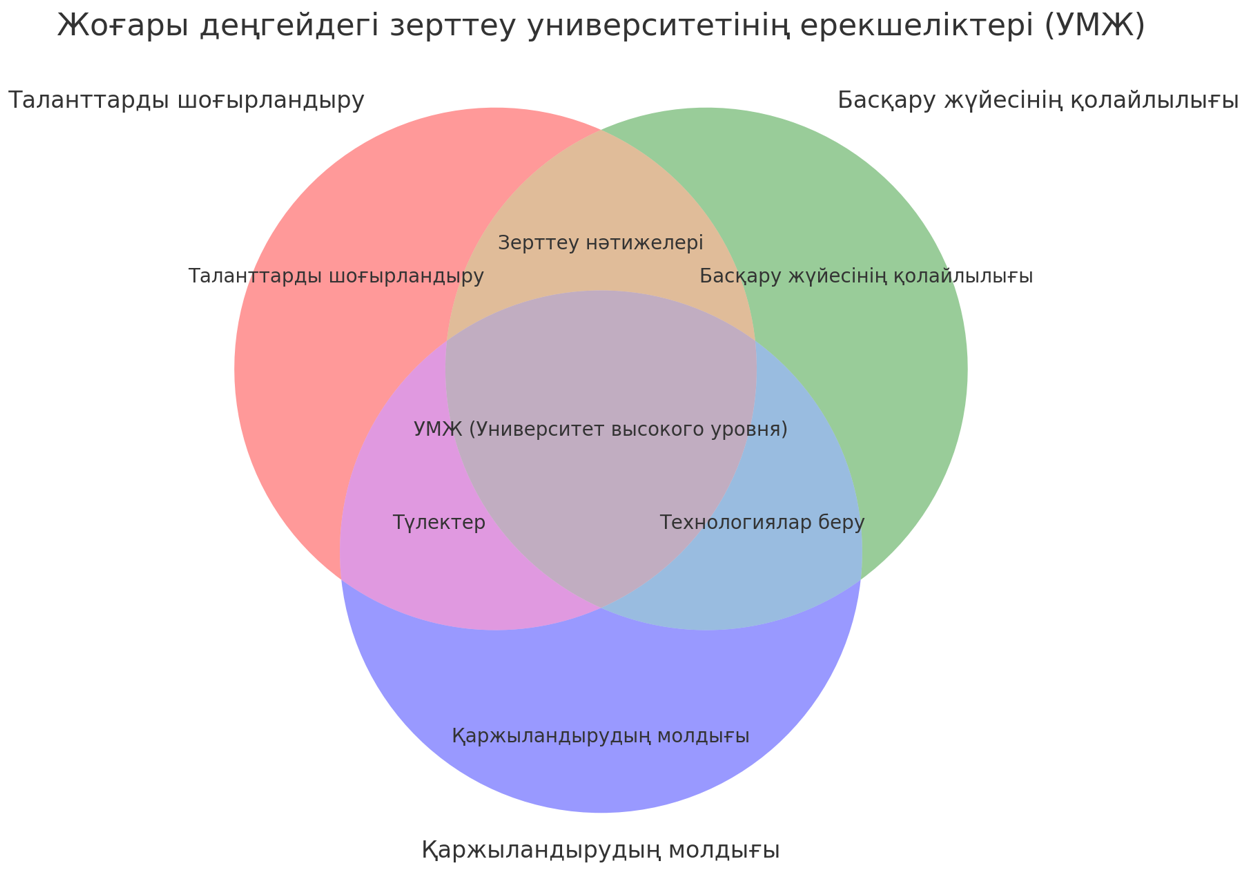
\includegraphics[width=0.8\textwidth]{media/ekon/image4}
	\caption*{1-сурет. Әлемдік деңгейдегі университеттің (УМЖ) сипаттамалары:
  негізгі факторлар}
\end{figure}


\begin{multicols}{2}

Бұл факторларға мыналар кіреді:

Профессорлық-оқытушылық құрам мен студенттер арасында жоғары
таланттардың концентрациясы;

Жетекші зерттеулерді жүргізуге және білім беру ортасын құруға мүмкіндік
беретін елеулі ресурстар;

Көшбасшылық қасиеттерді дамытуға, стратегиялық көрініс, инновациялар мен
икемділікті ынталандыратын және мекемелерге шешім қабылдауға және
ресурстарды басқаруға мүмкіндік беретін басқару ерекшеліктері.

Бұл үш топ факторларының белсенді өзара әрекеті жоғары деңгейлі зерттеу
университеттерінің ерекше ерекшелігі болып табылады. Әлемдік деңгейдегі
зерттеу университетінің рухы идеяларға ашықтықпен және дәстүрлі
түсініктерге сын тудыруға дайындықпен сипатталады.

Кәсіпкерлік қызметке бағытталған білім беруді қамтамасыз ететін
оқытушылардың мотивациясын қолдау мәселесі өзекті болып қала береді.
Білім берудегі жаңа стратегияларды дамыту негізгі стратегиялық ресурс --
оқытушылар құрамына байланысты. Жаңа білім беру бағдарламаларын құру
процесіне оқытушылардың қатысуын үздіксіз арттыруға ықпал ететін қолайлы
ортаны құруға барынша назар аудару қажет.

Барлық университеттерге әлемдік деңгейдегі жоғары деңгейге жету мүмкін
емес, өйткені сыртқы әлеуметтік, экономикалық, ақпараттық және құқықтық
факторлар үлкен әсер етеді, бірақ білім беру ұйымдарын басқаруға
заманауи кәсіпкерлік типтегі университеттерді сипаттайтын элементтерді
енгізу әбден мүмкін.

Кәсіпкерлік дағдысы басқаларға пайда келтіру үшін мүмкіндіктер мен
идеяларға сәйкес әрекет ету ретінде анықталды. Құрылатын құндылық
қаржылық, мәдени немесе әлеуметтік болуы мүмкін.

Қазақстандағы университеттік білім беруді дамытудың қазіргі кезеңі
қазіргі заманғы инновациялық және кәсіпкерлік университеттің оңтайлы
моделін белсенді іздеумен сипатталады. Қазақстандағы жоғары білім
берудің даму үрдістерін талдау кәсіпкерлік университеттерді қалыптастыру
процесі бастапқы кезеңде екенін көрсетеді.

Қазақстан жастары арасында инновациялық және кәсіпкерлік ойлауды
қалыптастыруда келесі сипаттамалар негіз болып табылады: кәсіпкерліктің
құндылығын, кәсіпкерлік ойлау стилін және қызмет түрін түсіну;
кәсіпкерлік ойлауды дамытатын білім мен дағдыларды алу; университет
ішінде және оның айналасында кәсіпкерлік экожүйесін қалыптастыру, оның
ішінде кадрлар, инфрақұрылым, оқиғалар ағымы.

Университеттерді жаңа типтегі ұйымдарға (кәсіпкерлік университеттерге)
айналдыру жолдары өзекті мәселе болып табылады, олар инновациялық
технологияларды, еңбек нарығын, ғылымды қажет ететін ғылыми жобаларды
дамытуға және басқаруға бағытталған.

Астана, Ақтөбе, Атырау университтерінде кәсіпкерлік орталығы жастар
арасында кәсіпкерлік ортаны дамыту және кәсіпкерлік қызметті танымал ету
бойынша жұмысты 2022 жылдың қаңтарынан бастап жүргізіп келеді. 2022
жылдың қыркүйегінен бастап Орталық құрылымында стартаптарды инкубациялау
өтетін «Startup » алаңы жұмыс істейді. Қазіргі уақытта инкубациялық
бағдарлама дайындалып, оған оқыту, тәлімгерлік, трекерлік қызметтер
кіреді. Инкубацияға іріктеу «Startup Fair» бизнес-идеялар конкурсы
форматында өтеді.

Астана, Ақтөбе, Атырау университтерінде кәсіпкерлікке қызығушылық
танытатын студенттерді анықтау үшін сауалнама жүргізілді, оған келесі
ашық сұрақтар енгізілді:

«``Кәсіпкерлік ойлау'' дегенді сіз қалай түсінесіз, 2-3 сөйлеммен
сипаттаңыз.»

«Университетте кәсіпкерлік құзыреттіліктерді дамыту мүмкіндіктерін қалай
көресіз, 2-3 сөйлеммен сипаттаңыз.»

«Өз бизнес-жобаңызды қай салада жүзеге асырғыңыз келеді?»

«Сіз білетін кәсіпкерлерді атаңыз (қызмет саласын көрсете отырып).»

«Сіз тәуекелге қалай қарайсыз?»

Сауалнама Астана, Ақтөбе, Атырау университтерінде барлық курс
студенттеріне 2023-2024 оқу жылының бірінші семестрінде ұсынылды.
Жауаптар 532 респонденттен алынды және жас, жыныс, оқу ақысының түрі,
мамандық критерийлері бойынша әртүрлі пропорцияларда бөлінді (1-кесте).
\end{multicols}

{\bfseries 1-кесте. Сауалнамаға қатысқан студенттердің ұжымдық портреті}

% \begin{longtable}[]{@{}
%   >{\raggedright\arraybackslash}p{(\columnwidth - 2\tabcolsep) * \real{0.7037}}
%   >{\raggedright\arraybackslash}p{(\columnwidth - 2\tabcolsep) * \real{0.2963}}@{}}
% \toprule\noalign{}
% \begin{minipage}[b]{\linewidth}\raggedright
% Сипаттама
% \end{minipage} & \begin{minipage}[b]{\linewidth}\raggedright
% \%
% \end{minipage} \\
% \midrule\noalign{}
% \endhead
% \bottomrule\noalign{}
% \endlastfoot
% Жасы
% 
% - 16-17
% 
% - 18-19
% 
% - 20-21
% 
% - 22 жастан үлкен & 30
% 
% 37
% 
% 32
% 
% 1 \\
% Жынысы
% 
% - әйел
% 
% - ер & 60
% 
% 40 \\
% Оқу бюджеті
% 
% - мемлекеттік грант негізде
% 
% -ақылы негізде & 58
% 
% 42 \\
% Мамандану
% 
% - техникалық
% 
% - гуманитарлық & 47
% 
% 53 \\
% Ескерту:Автормен құрастырылған & \\
% \end{longtable}

\begin{multicols}{2}

Алынған мәліметтерді өңдеудің бірінші кезеңінде студенттердің
кәсіпкерлік ойлау туралы кешенді түсінігін анықтау үшін семантикалық
талдау жүргізілді.

1-ші сұраққа жауап беру кезінде жиі айтылған сөздер: «тәуекел» (75
жауап), «қабілет» (57), «мақсат» (53), «пайда» (12), «шешім» (47),
«бизнес» (49), «пайда» (31) және т.б. Ең жиі кездесетін екі сөзден
тұратын тіркестер: «пайда табу» (29), «көшбасшылық қасиеттер» (27),
«мақсатқа жету» (18), «тәуекел деңгейі» (17).

2-ші сұраққа жауаптарда студенттердің басым бөлігі (85\%) келесі білім
беру ортасының элементтерін атап өтті: «жоба» (86 жауап), «қызмет» (72),
«бизнес» (87). Оқушылардың жобалық қызметті жүзеге асыру мүмкіндігін
нақты түсінуі оң нәтиже болып табылады, алайда басқа құралдар бойынша
студенттердің ақпараты аз екендігі анықталды.

3-ші сұраққа жауаптарда студенттердің бизнес түрлері бойынша таңдаулары
өте кең болды және көбінесе таңдалған сала оқу мамандығына сәйкес келді:
IT, электр энергетикасы, білім беру қызметтері, дизайн, психология,
аударма ісі және т.б. 4-ші сұраққа жауаптарда студенттер жиі атап өткен
кәсіпкерлер: Уоррен Баффет (107 жауап), Илон Маск (73), Марк Цукерберг
(62), Джек Ма (37), Билл Гейтс (20), Джефф Безос (19), Маргулан
Сейсембай (6) және т.б.

5-ші сұраққа жауап берген студенттердің 9,5\% тәуекелге теріс көзқарас
білдірсе, 81,5\% респонденттер бұл фактордың кәсіпкерлік қызметтің
міндетті сипаттамасы екенін түсінеді. Алынған ақпарат білім беру
мазмұнын студенттердің қызығушылықтарын дәлірек ескеретіндей етіп
дайындауға мүмкіндік береді, бұл олардың тиісті оқу және ағартушылық
курстарға деген қызығушылығын арттырады.

Алынған мәліметтерді өңдеудің екінші кезеңінде кәсіпкерлік бағытқа
қызығушылық танытатын студенттер анықталды, олар келесі критерийлер
бойынша таңдалды:

\begin{itemize}
\item
  кәсіпкерлік мінез-құлық моделіне қатысты жеке пікірі бар;
\item
  университеттің білім беру ортасында кәсіпкерлік қабілеттерін дамыту
  мүмкіндіктерін көреді;
\item
  өз бизнес жобасын қай салада жүзеге асыратынын біледі;
\item
  кәсіпкерлік ортадан кемінде екі өкілді саласын көрсете отырып атай
  алады;
\item
  тәуекелге оң немесе бейтарап көзқараспен қарайды.
\item
  Алынған мәліметтерге сәйкес, анықталған талаптарға сәйкес келетін 241
  респондент бар, бұл жалпы санының 29,4\%-ын құрайды, олардың 69\%-ы
  әйелдер, 31\%-ы ерлер; 77\%-ы гуманитарлық мамандықтарда оқиды (оның
  ішінде 59\%-ы экономикалық мамандықтар бойынша студенттер), 85,7\%-ы
  16-18 жас аралығында.
\end{itemize}

Сауалнама барысында респонденттердің 81\%-ы жастар кәсіпкерлігін дамыту
үшін арнайы даму/қолдау бағдарламалары қажет екенін атап өтті, оларды
мемлекеттік/қоғамдық/коммерциялық құрылымдар жүзеге асыруы керек.

Зерттеу барысында жастардың көпшілігі кәсіпкерлік қызметті жүргізу
шарттары алдағы 1-2 жылда жақсарады деп санайтыны (56,5\%), 30\%-ы
шарттар өзгермейді деп санайды және тек 8,8\%-ы кәсіпкерлік қызмет
шарттары нашарлайды деп санайды. Сонымен қатар, келесі бірнеше жылда
мақсатты аудиторияның 61\%-ы жалғыз немесе басқалармен бірге кәсіпкерлік
қызметті, оның ішінде кез келген өзін-өзі жұмыспен қамту түрін бастай
алады деп анықталды.

Осылайша, әртүрлі бағыттарда оқитын студенттердің шамамен 50\%-ы
кәсіпкерлік ойлауды дамытуға қызығушылық танытады. Кәсіпкерлік өзін-өзі
анықтауға және бизнес-жобаларды жасау, әзірлеу және іске асыру бойынша
міндеттерді жүзеге асырудың нақты тәжірибесін алуға жағдай жасайтын
білім беру ортасын қалыптастыру кәсіби білім берудің өзекті міндеті
болып табылады.

Осы зерттеу аясында қарастырылатын мәселелердің бірі - оқыту барысында
немесе университетті бітіргеннен кейін студенттерді кәсіпкерлік қызметке
тарту процесі. Зерттеу барысында университеттің кәсіпкерлік
инфрақұрылымын дамыту студенттердің кәсіпкерлік ниетінің пайда болуына
және олардың өз бизнесін құру және дамыту аясында одан әрі жүзеге
асырылуына әсер ететін маңызды фактор бола алатыны анықталды.
Жүргізілген зерттеу нәтижелеріне сүйене отырып, студенттерде
экономикалық ойлау мен кәсіпкерлік қызмет дағдыларын қалыптастыру үшін
бес аспектіні бір мезгілде дамыту қажет екенін атап өтуге болады
(2-кесте).
\end{multicols}

{\bfseries 2-кесте. Жастар арасында кәсіпкерлік ойлауды дамытатын негізгі
факторлар}

% \begin{longtable}[]{@{}
%   >{\raggedright\arraybackslash}p{(\columnwidth - 8\tabcolsep) * \real{0.2208}}
%   >{\raggedright\arraybackslash}p{(\columnwidth - 8\tabcolsep) * \real{0.2344}}
%   >{\raggedright\arraybackslash}p{(\columnwidth - 8\tabcolsep) * \real{0.1964}}
%   >{\raggedright\arraybackslash}p{(\columnwidth - 8\tabcolsep) * \real{0.1793}}
%   >{\raggedright\arraybackslash}p{(\columnwidth - 8\tabcolsep) * \real{0.1691}}@{}}
% \toprule\noalign{}
% \begin{minipage}[b]{\linewidth}\raggedright
% Институционалды
% \end{minipage} & \begin{minipage}[b]{\linewidth}\raggedright
% Мемлекеттік
% \end{minipage} & \begin{minipage}[b]{\linewidth}\raggedright
% Білім беру
% \end{minipage} & \begin{minipage}[b]{\linewidth}\raggedright
% Қоршаған орта
% \end{minipage} & \begin{minipage}[b]{\linewidth}\raggedright
% жеке
% \end{minipage} \\
% \midrule\noalign{}
% \endhead
% \bottomrule\noalign{}
% \endlastfoot
% \begin{minipage}[t]{\linewidth}\raggedright
% \begin{itemize}
% \item
%   кәсіпкерлікке қолайлы жағдай жасау
% \item
%   кәсіпкерлік мәдениетті дамыту
% \end{itemize}
% \end{minipage} & \begin{minipage}[t]{\linewidth}\raggedright
% \begin{itemize}
% \item
%   ресурстарға қолжетімділік
% \item
%   қолдау бағдарламаларын дамыту
% \item
%   әкімшілік кедергілерді азайту
% \end{itemize}
% \end{minipage} & \begin{minipage}[t]{\linewidth}\raggedright
% \begin{itemize}
% \item
%   оқытудың жаңа тәсілдері
% \item
%   оқу-әдістемелік материалдарды жаңарту
% \end{itemize}
% \end{minipage} & \begin{minipage}[t]{\linewidth}\raggedright
% \begin{itemize}
% \item
%   кәсіпкерлік бастамаларды қолдау
% \item
%   капитал беру
% \end{itemize}
% \end{minipage} & \begin{minipage}[t]{\linewidth}\raggedright
% \begin{itemize}
% \item
%   ішкі мотивация\\
%   білім мен ресурстар жинақтау
% \item
%   өзін-өзі жүзеге асыру
% \end{itemize}\strut
% \end{minipage} \\
% \multicolumn{5}{@{}>{\raggedright\arraybackslash}p{(\columnwidth - 8\tabcolsep) * \real{1.0000} + 8\tabcolsep}@{}}{%
% Ескерту: мәліметтер негізінде автормен құрастырылған} \\
% \end{longtable}

\begin{multicols}{2}

Сарапшылардың пікірінше, жастар арасында кәсіпкерлік қызметті бастаудың
ынталандырушы факторлары:

\begin{enumerate}
\def\labelenumi{\arabic{enumi}.}
\item
  Кәсіпкерлікті дамыту бойынша мемлекеттік бағдарламалардың болуы;
\item
  Білім алу және кейіннен бизнесті ашуға арналған оқыту
  бағдарламаларының болуы;
\item
  Болашақ кәсіпкерлердің жақын ортасында табысты кәсіпкерлік қызметтің
  үлгілерінің болуы.
\end{enumerate}

Фокус-топ қатысушыларының пікірінше, кәсіпкерлік қызметті бастауға ықпал
ететін негізгі факторлар мыналар:

\begin{itemize}
\item
  қаржылық тәуелсіздік;
\item
  инновациялық идея;
\item
  хобби;
\item
  көп табыс табуға ұмтылыс (3-кесте).
\end{itemize}
\end{multicols}

{\bfseries 3-кесте. Кәсіпкерлік қызметпен айналысуға ынталандыратын негізгі
себептер}

% \begin{longtable}[]{@{}
%   >{\raggedright\arraybackslash}p{(\columnwidth - 2\tabcolsep) * \real{0.7500}}
%   >{\raggedright\arraybackslash}p{(\columnwidth - 2\tabcolsep) * \real{0.2500}}@{}}
% \toprule\noalign{}
% \begin{minipage}[b]{\linewidth}\raggedright
% Қаржылық тәуелсіздік
% \end{minipage} & \begin{minipage}[b]{\linewidth}\raggedright
% 65\%
% \end{minipage} \\
% \midrule\noalign{}
% \endhead
% \bottomrule\noalign{}
% \endlastfoot
% Біреуге жұмыс жасағысы келмеу & 44\% \\
% Көбірек ақша табу & 48\% \\
% Жақсы бизнес идея & 29\% \\
% Имидж & 27\% \\
% Тәжірибе & 25\% \\
% Амбицияны жүзеге асыру & 23\% \\
% Әлеуметтік мәселелерді шешу & 19\% \\
% Басқа мақсаттар & 17\% \\
% \end{longtable}

\begin{multicols}{2}

Кәсіпкерлік қызметтің негізгі тартымды жағы жастар үшін еркіндік болып
табылады -- шешім қабылдауда дербестік, шығармашылық және меншік иесіне
тәуелділіктің болмауы. Зерттеу нәтижелері қазіргі жастардың
кәсіпкерлікке, өз ісін ашуға белгілі бір қызығушылығы бар екенін
көрсетеді. Өзінің кәсіпкерлік қызметі арқылы жастар лайықты материалдық
жағдайға қол жеткізуді және бар идеялары мен амбицияларын жүзеге асыруды
жоспарлап отыр.

Жастардың өзін-өзі бағалауы, қоғамдық пікір және жеке тұлғаның
әлеуметтік байланыстары кәсіпкерлікті қызмет түрі ретінде таңдауға
айтарлықтай әсер етуі мүмкін.

Жас кәсіпкерлерге ел, аймақ, университет немесе отбасы ортасында
қолжетімді ресурстарды елемеуге болмайды және олардың өз қабілеттерін де
назардан тыс қалдырмауы маңызды. Әсіресе әлеуметтік капиталдың барлық
түрлерін, яғни отбасынан және университеттен қолжетімді қолдауды дамыту
өте маңызды, өйткені дәл осы қолдау жаңа кәсіпорынды іске қосу үшін
бұрын қолжетімсіз ресурстарға қол жеткізуге мүмкіндік береді.
Университеттік және отбасылық қолдаудың әртүрлі формаларын пайдалану жас
кәсіпкерлер үшін маңыздырақ, сондықтан оларға көбірек назар аудару және
оларды пайдалану қажет.

Қазақстанның қазіргі заманғы жоғары оқу орындары кәсіпкерлік ойлауды
ынталандыруға бағытталған жаңашыл оқыту әдістерін белсенді түрде
енгізуде. Негізгі сәттердің бірі практикалық сабақтар мен жобалық
жұмысты оқу процесіне енгізу болып табылады. Студенттерге өз
бизнес-жоспарларын, өнімдер мен қызметтердің прототиптерін әзірлеуге,
сондай-ақ олардың нарықтық әлеуетін бағалауға мүмкіндік беріледі.

Хакатондар, стартап-байқаулар, инкубаторлар мен акселераторлар сияқты
бастамалар кәсіпкерлік ойлауды дамытуда маңызды рөл атқарады. Бұл
іс-шаралар студенттердің білімдерін тәжірибеде қолдануына ғана емес,
сонымен қатар жас кәсіпкерлердің қауымдастығын құруға, тәжірибе және
идеялар алмасуға ықпал етеді.

Әлемдік кәсіпкерлік және білікті кәсіпкерлерді оқыту саласының дамуын
қадағалай отырып, кәсіпкерлік қызметтің негізі халыққа ерте жастан
бастап қаланған елдерді атап өтуге болады. Сондықтан кәсіпкерлік ойлауды
балабақшадан бастап оқыту жүйесін енгізу ұсынылады.

{\bfseries Қорытынды.} Қазіргі уақытта кәсіпкерлік тұлғаны қалыптастырудағы
инновациялық тәсіл ғана Қазақстанға жаңа инновациялық секірісті жүзеге
асыруға, ұлттық экономиканы жаһандық сын-қатерлерді ескере отырып
модернизациялау мүмкіндігіне ие болуға мүмкіндік береді.

Кәсіпкерлік ойлау жүйесінің заманауи білім беру жүйесі XXI ғасырдың
сын-қатерлеріне жауап беруі керек және бизнес жүргізу дағдыларын
қалыптастыруға бағытталуы тиіс. Бұл дағдылар келесі басым инновациялық
салалардың әлемдік даму үрдістерін ескере отырып қалыптастырылуы керек:

Өмір туралы ғылымдар;

Ақпараттық-телекоммуникациялық жүйелер;

Наносистемалар индустриясы;

Қоршаған ортаны ұтымды пайдалану;

Көлік және ғарыш жүйелері;

Энергия тиімділігі, энергия үнемдеу, ядролық энергетика.

Қазақстан жастары арасында кәсіпкерлік ойлауды дамыту үшін келесі
шараларды жүзеге асыру ұсынылады:

Технопарктер, бизнес-инкубаторлар, кәсіпкерлікті қолдау орталықтарының
жұмыстарын жандандыру, жастар жобаларын кеңес беру, талқылау және
бизнесте енгізу үшін «алаңдар» құру;

Табиғи және техникалық ғылымдар саласында халықаралық жастар
ғылыми-технологиялық паркін ұйымдастыру, онда әлемдік тәжірибені ескере
отырып, инновациялық өнімдерді әзірлеу және оларды инновациялық бизнеске
интеграциялау мүмкін болады;

Студенттердің инновациялық кәсіпкерлігін дамытуға академиялық және
салалық ғылымды тарту (студенттердің тәжірибеден өтуі, студенттік
инновациялық бизнес-идеяларды коммерцияландыру мақсатында қарастыру және
т.б.);

Білім мен дағдыларды параллельді түрде меңгеру, бекіту және нақты бизнес
жобаларды жүзеге асыру арқылы дамытуға негізделген оқыту моделін орнату
(студенттердің жеке өсуі).

Қорытындылай келе, кәсіпкерлікті қалыптастыру және дамыту Қазақстан
Республикасында экономикалық реформаларды жүзеге асырудың заңды процесі
болып табылатынын атап өту керек. Бизнесті дамыту оның қатысушыларынан
жаңа мамандықтарды, жаңа тәсілдерді және жаңа білімдерді игеруді талап
етеді. Қазақстан экономикасының даму жағдайында білім беру мазмұнының
қоғам қажеттілігіне сәйкес келуі маңызды, яғни әртүрлі нарықтық
жағдайларда жылдам бейімделуге қабілетті, бастамашыл, экономикалық
сауатты, кәсіби білімді кәсіпкерлердің жаңа түрін қалыптастыру қажет.

Жастар арасында кәсіпкерлік ойлауды дамыту, оларды кәсіпкерлік қызметке
тарту --- бұл тек шағын бизнестің үлесін арттыру және құрылымын жақсарту
ғана емес, сонымен қатар, олардың жұмыспен қамту мәселесін шешу,
шығармашылық әлеуетін және кәсіби амбицияларын жүзеге асыру, қоғамның
тұрақтылығын қамтамасыз ету болып табылады.
\end{multicols}


\begin{center}
  {\bfseries Әдебиеттер}
  \end{center}
  
  \begin{references}

\begin{enumerate}
\def\labelenumi{\arabic{enumi}.}
\item
  Javeed, A., Aljuaid, M., Mehmood, S., Khan, M Y., Mahmood, Z., Shahid,
  D., \& Wali, S S. Factors affecting youth empowerment and
  entrepreneurial initiatives: Social implications and way forward //
  Frontiers Media. -2022. -Vol. 13.
  \href{https://doi.org/10.3389/fpsyg.2022.912259}{DOI
  10.3389/fpsyg.2022.912259}
\item
  Chiru, C., Tăchiciu, L., \& Ciuchete, S G. Psychological Factors,
  Behavioural Variables and Acquired Competencies in Entrepreneurship
  Education // Elsevier BV. -2012.-Vol. 46.- P. 4010-4015.
  \href{https://doi.org/10.1016/j.sbspro.2012.06.188}{DOI
  10.1016/j.sbspro.2012.06.188}
\item
  Alaref, J J S., Brodmann, S., \& Premand, P. The medium-term impact of
  entrepreneurship education on labor market outcomes: Experimental
  evidence from university graduates in Tunisia // Elsevier BV. -2020.-
  Vol. 62.- P.101787-101787.
  \href{https://doi.org/10.1016/j.labeco.2019.101787}{DOI
  10.1016/j.labeco.2019.101787}
\end{enumerate}

Rohim, A., Diana, I N., \& Rofiq, A. Development of the Students'
Entrepreneurship in Building a Creative Economy. -2021. -Vol. 4(1).-P.
123-131. DOI
\href{https://doi.org/10.31538/iijse.v4i1.1555}{10.31538/iijse.v4i1.1555}

\begin{enumerate}
\def\labelenumi{\arabic{enumi}.}
\setcounter{enumi}{3}
\item
  Stabingis, L., \& Raupelienė, A. Factors influencing entrepreneurial
  intentions among the students in the baltic sea region countries //
  Vilnius Gediminas Technical University.-2023. -Vol. 24(1).- P.
  301-311. DOI
  \href{https://doi.org/10.3846/btp.2023.18948}{10.3846/btp.2023.18948}
\item
  Taubayev, А., Kamenova, A., Legostayeva, A., Srailova, G., \&
  Ayazhanov, K. Innovative entrepreneurship development: main problems
  and educational limitations in Kazakhstan. -2019. -Vol. 177(5-6). -P.
  92-100. \href{https://doi.org/10.21003/ea.v177-08}{DOI
  10.21003/ea.v177-08}
\item
  Abdikerova, G O., Kylyshbaeva, B., Duisenova, S., \& Altynbekov, A.
  Quality Education as a Basis for Professional Mobility of Youth in the
  Republic of Kazakhstan // Elsevier BV. -2014.-Vol.116.- P. 4487-4492.
  \href{https://doi.org/10.1016/j.sbspro.2014.01.972}{DOI
  10.1016/j.sbspro.2014.01.972}
\item
  Bosman L., Fernhaber S. Teaching the Entrepreneurial Mindset Across
  the University. An Integrative Approach. Springer Cham, 2021. 135 p.
  DOI 10.1007/978-3-030-79050-9
\item
  Khamzina, Z A., Buribayev, Y A., Yermukanov, Y., \& Alshurazova, A. Is
  it possible to achieve gender equality in Kazakhstan: Focus on
  employment and social protection // SAGE Publishing. -2020.- Vol.
  20(1).- P. 5-20. \href{https://doi.org/10.1177/1358229120927904}{DOI
  10.1177/1358229120927904}
\item
  Kaldybayeva, O V., Ashimkhanova, D E., Baigabylov, N O., Tagayeva, S
  B., Mukhambetova, K., \& Manzhugulova, A Y. Youth installations to
  labour in modern Kazakhstan. Inderscience
  Publishers.-2018.-Vol.10(4).-P.325-345.
  \href{https://doi.org/10.1504/ijlc.2018.095817}{DOI
  10.1504/ijlc.2018.095817}
\item
  Mueller, S L., Thomas, A S., \& Jaeger, A M. National entrepreneurial
  potential: The role of culture, economic development, and political
  history // Elsevier BV. -2002. - P. 221-257.
\end{enumerate}

DOI 10.1016/s0747-7929(02)14037-6

\begin{enumerate}
\def\labelenumi{\arabic{enumi}.}
\setcounter{enumi}{10}
\item
  Larin M.V.,Мukhatova О.Functional requirements for information systems
  electronic document circulation//Journal of History-2019.-Vol.
  92(1).-P 55-61. \href{https://doi.org/10.26577/jh-2019-1-411}{DOI
  10.26577/jh-2019-1-411}
\end{enumerate}
\end{references}
\begin{authorinfo}

  \hspace{1em}\emph{{\bfseries Авторлар туралы мәліметтер}}

Сайымова М.Д. -PhD, қауымдастырылған профессор, Ақтөбе өңірлік
университеті. Қ. Жұбанова, Ақтөбе, Қазақстан, e--mail:
\href{mailto:77mika-07@mail.ru}{msaiymova@zhubanov.edu.kz};

Мауина Ғ.А. -Экономика ғылымдарының кандидаты, қауымдастырылған
профессор, С. Сейфуллин атындағы

Қазақ агротехникалық зерттеу университеті, Астана, Қазақстан, е-mail:
\href{mailto:mauina_galiya@mail.ru}{\nolinkurl{mauina\_galiya@mail.ru}};

Байдалинова А.С. -PhD, С. Утебаев атындағы Атырау мұнай және газ
университеті, Атырау, Қазақстан, е-mail: aynur.sultanovna@mail.ru;

Сағындықова Г.М.-Экономика ғылымдарының кандидаты, қауымдастырылған
профессор, Қ.Құлжанов атындағы Қазақ технология және бизнес
университеті, Астана, Қазақстан, e-mail:
\href{mailto:gsmaktobe1@mail.ru}{\nolinkurl{gsmaktobe1@mail.ru}}

\hspace{1em}\emph{{\bfseries Information about the authors}}

Saiymova М.D. -PhD, Assistant Professor, Aktobe Regional University
named after K. Zhubanov, Акtobe, Kazakhstan, e--mail:
msaiymova@zhubanov.edu.kz;

Mauina G.A. - Candidate of Economic Sciences, an associate professor, S.
Seifullin Kazakh Agro Technical Research University, Astana, Kazakhstan,
e-mail:
\href{mailto:mauina_galiya@mail.ru}{\nolinkurl{mauina\_galiya@mail.ru}};

Baidalinova A.S. -PhD Atyrau Oil and Gas University named after S.
Utebayev, Atyrau, Kazakhstan,

e-mail: aynur.sultanovna@mail.ru;

Sagindykova G.M. -candidate of economic sciences, associate professor,
K.Kulazhanov kazakh university of technology and business, Astana,
Kazakhstan, e-mail: gsmaktobe1@mail.ru

\end{authorinfo}
